\section{Critiques of FortNOX and Implementation Challenges}
\label{sec:critique}
In designing our implementation of alias reduced rules for rule conflict detection, we encountered a number of apparent shortcomings and blind spots in the FortNOX implementation that would still allow a subversive application to insert conflicting rules without detection. Our critiques, and the corresponding challenges are detailed below.

Note that all of our critiques are based solely on the information provided in \cite{Porras:2012:SEK:2342441.2342466}, as the reference implementation of FortNOX was never made public due to concerns about its viability and completeness.\footnote{We confirmed this in communication with FortNOX author Phil Porras.} A reference implementation of SE-Floodlight (secure Floodlight) by the same authors, has been proposed for release in summer 2013. While it is possible that SE-Floodlight will address our concerns, there is currently no implementation available on which to base more specific critiques.

\subsection{Controller-Based Rule Evasion}
As we mentioned in section \ref{subsec:cbre}, FortNOX does not prevent controller based rule evasion.
We found this to be a major shortcoming since this allows an application to subvert any rule in a switch's flow table.
A malicious application doesn't even need a dummy host in place to perform this attack.
Floodlight-CD prevents this by checking \texttt{PACKET\_OUT} messages in addition to flow rules before forwarding a packet to a switch. 
%FortNOX only focuses on examining and filtering out conflicting \emph{flow rules} from being inserted into switches. 
%However, packet rewriting and manipulation is not limited to flow rules inserted into the switches themselves. 
%Rules can be inserted that, when matched, forward the packet to the controller. 
%This can happen because a new flow has arrived at a switch for which there is not yet a corresponding flow rule, or because an idle or hard timeout means that a previous flow rule has been discarded from the switch. 
%At this point, a subversive application can arbitrarily rewrite a packet \emph{in the controller} in order to subvert rules, before sending it back to the switch to be forwarded. 
%Even if another application in the controller installs a corresponding rule during the same session in the controller, the damage has already been done. 

%In order to defend against malicious flow subversion at the controller level, our implementation examines the actions of both attempted flow-table insertions, and of \texttt{PACKET\_OUT} events. That is, we examine outgoing packets to see if they conflict with any of our alias reduced rules in our in-memory mapping of allowed actions. This prevents malicious actions by applications both at the flow-rule level and the controller level.

\subsection{Malicious Tunneling Across Switches}
Another substantial issue with the FortNOX approach is that it only verifies that a candidate rule is not in conflict with the current rule set of a \emph{single} switch. 
Enforcement at the level of a single switch is sufficient only to thwart the simplest attacks, such as the single-rule dynamic tunneling attack outlined above in \ref{subsec:arr}. 
However, when a Floodlight application can install rules into multiple switches and/or manipulate packets flowing through multiple switches, installing a candidate ARR requires verifying that its installation would not create a flow that would subvert any existing flow restrictions throughout the network. 
In other words, to adequately protect the \emph{network}, enforcement must be considered on the level of the whole network, not just a single switch.

\begin{figure*}[ht!]
	\begin{center}
		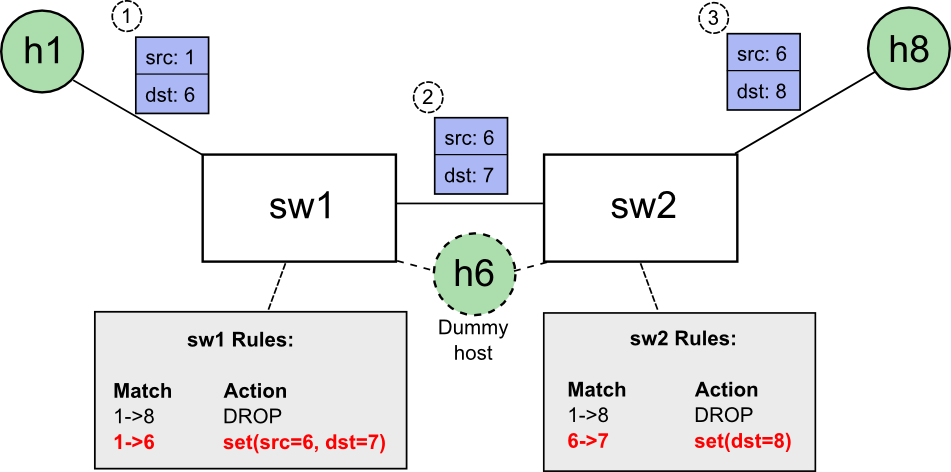
\includegraphics[width=\columnwidth]{figs/multiSwitch_diagram.png}
		\caption{Dynamic flow tunneling using multiple switches.}
		\label{fig:dft_multi}
	\end{center}
\end{figure*}

Consider a simple extension to the dynamic tunneling attack, depicted in figure \ref{fig:dft_multi}, where the legitimate rule is once again $(h1) \Rightarrow (h8:80): DROP$. 
Then the subversion rules would be as follows: 

\begin{align}
  Sw1: (h1) \Rightarrow (h6): set(src=h6, dest=h7) \\
  Sw1: (h7) \Rightarrow (h6): set(src=h6, dest=h1) \\
  Sw2: (h6) \Rightarrow (h7): set(dest=h8) \\
  Sw2: (h8) \Rightarrow (h6): set(src=h7)
\end{align}

Assuming the malicious application installs each of these rules in turn, each is considered as a candidate ARR (cARR) and checked pairwise against existing rules according to the procedure described in section \ref{subsec:conflict} above. 
Recall that the algorithm builds the union of source and destination rules and actions between the cARR and each fARR in the flow table, and detects a conflict if actions differ and the intersection of the sources and destinations of the ARRs are non-empty. 
In this case though, testing the insertion of the rules into Sw1 would yield a empty destination set since \texttt{h8} does not appear in the cARRs' destination sets. 
Similarly, \texttt{h1} does not appear in the cARRs' source sets for the rules inserted into Sw2, so they would be inserted successfully. 

Like FortNOX, Floodlight-CD does not prevent tunneling across multiple switches.
We explore the challenges and possible solutions to this problem in the next section.


%Instead of simply checking each cARR pairwise against each fARR \emph{only} for the target switch's alias rule set and rejecting or accepting the cARR at that stage, the algorithm can continue to build a \emph{complete union set} (CUS) across the alias rule sets of all switches in a potential flow's forwarding path, taking into account the potential ramifications of the insertion of each candidate rule into each switch. 
%At the end, we would reject a candidate rule if and only if the intersection of the CUS and fARR destination and source sets are both non-empty. 

